\chapter[Resultados Parciais]{Resultados Parciais}

\section{Protótipo inicial}

A fim de atestar a viabilidade do porte do jogo \textit{Traveling Will}, desenvolvido inicialmente para PC, para a plataforma \textit{Nintendo Game Boy Advance}, foi feita uma versão funcional do menu original do jogo, tendo essa versão sido testada em um GBA real. Para isso, a principal ferramenta utilizada foi a libtonc \cite{libtonc}, que nessa versão inicial fez o papel de engine do jogo.

Abaixo é possível comparar o menu principal do jogo original com o protótipo implementado sendo executado em um emulador de \textit{Game Boy Advance}:

\begin{figure}[H]
 \centering \includegraphics[keepaspectratio=true,scale=0.6]{figuras/tw-original-1.eps}
   \caption{Jogo original \textit{Traveling Will} sendo executado em um PC}
   \makebox[\width]{Fonte: \textit{Autores}.}
   \label{tw-original-1}
\end{figure}

\begin{figure}[H]
 \centering 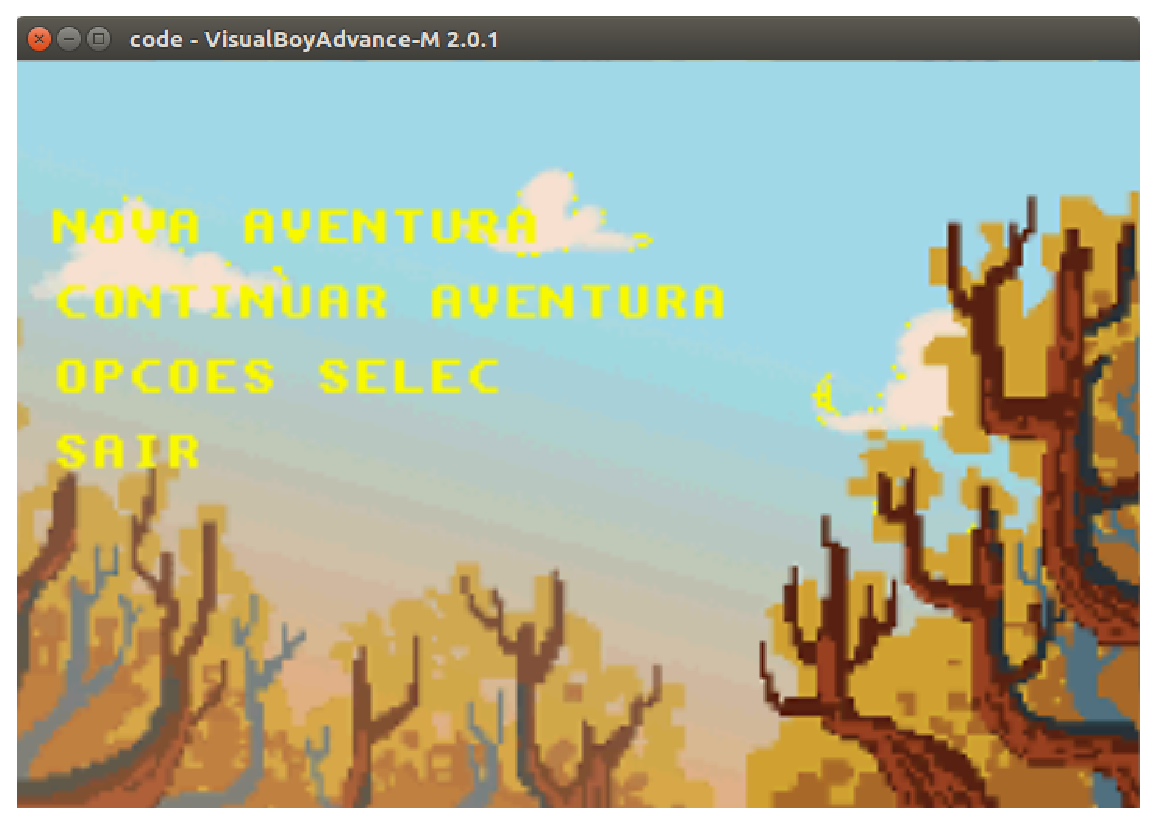
\includegraphics[keepaspectratio=true,scale=0.6]{figuras/tw-gba-1.eps}
   \caption{Protótipo implementado sendo executado em um emulador de GBA}
   \makebox[\width]{Fonte: \textit{Autores}.}
   \label{tw-gba-1}
\end{figure}

\section{Desenvolvimento da \textit{engine}}

Após a finalização do protótipo inicial, foi iniciado o desenvolvimento da engine que irá substituir a libtonc na versão final do jogo. Ela irá padronizar a utilização dos recursos providos pelo GBA e irá conter um módulo de vídeo, áudio, \textit{input}, física, dentre outros.

Até o momento, o módulo de \textit{input} e parte do módulo de vídeo foram implementados.

\subsection{Módulo de \textit{input}}

  TODO

  explicar pra quê serve e explicar funcionamento

  botar código

  botar print da demo dos botões

  \subsubsection{Método para checagem dos estados dos botões}

\subsection{Módulo de vídeo}

  \subsubsection{Método para definição do modo de vídeo}

  TODO

  explicar pra quê serve e explicar funcionamento

  botar código

  \subsubsection{Método para definição da camada em que será inserida a imagem de fundo}

  TODO

  explicar pra quê serve e explicar funcionamento

  botar código

  \subsubsection{Método para inserção da imagens}

TODO

explicar pra quê serve e explicar funcionamento

botar código

botar print da imagem no emulador